\newcommand{\xseen}{x^{\text{S}}}
\newcommand{\xfillzero}{\bar{x}}

\section{Methods}
In order to develop probabilistic models for irregular time series with arbitrary missingness, let us define some essential notation. First, for a given time $t$, let $\xseen_t$ denote the subset of all entries of $x_{t} \in \mathbb{R}^D$ that are \emph{seen} or present, not missing. $\xseen_t$ may vary in size depending on how many entries are missing at time $t$.  Second, let $\bar{x}_{t}$ be a vector of size $D$ constructed from $x_t$ by filling any missing entry with a numerical zero, but otherwise leaving present entries alone. Recalling that $s_t$ is a binary vector indicating the seen entries of $x_t$, we can write $\xfillzero_t \gets x_{t} \odot s_{t}$ to represent the element-wise product (denoted $\odot$) which fills any missing entry with zero.


\subsection{CRU model for seen features only}
\label{sec:CRU_gen_model_from_prev_work}

\citet{schirmer2022modeling} provide the following generative model for $\mathbf{\xseen}$, the \emph{seen} (non-missing) entries of the $D$-dimensional time series $\mathbf{x}$:
\begin{align}
    p( \mathbf{\xseen} ) &= \prod_{t \in \Gamma} p( \xseen_t | \{  \xseen_u : u < t, u \in \Gamma \} ),
    \\ \notag 
    &= \prod_{t \in \Gamma} \prod_{d : s_{td}=1} \mathcal{N}( x_{td} \mid h_{td}, \tau_{td}^2 ),
\end{align}
where $h_t, \tau_t$ are the decoded data representations for time $t$ produced by a CRU given zero-filled input:  $[h_{t_1}, \ldots], [\tau_{t_1}, \ldots] \gets \textsc{CRU}( \bar{x}_{t_1}, \ldots \bar{x}_{t_L}, \Gamma )$. Symbol $\mathcal{N}$ is the Gaussian pdf.

While this model can be fit on irregular time series with arbitrary missingness, we stress that it does not model the missingness indicator $s_t$ as a random variable and thus cannot account for data-dependent missingness mechanisms. Our later experiments show that in both synthetic  and real-world missingness scenarios, this leads to poor recovery of the underlying model and high error in extrapolation.

\subsection{CRU-FM generative model}
\label{sec:CRU_gen_model}
To better capture data-dependent missingness, we propose a generative model of both 
seen features $\mathbf{\xseen}$ and binary seen/missing indicators $\mathbf{s}$ over time. We call this the CRU-FM, emphasizing the joint modeling of both Features and Missingness, and illustrate this model in Fig.~\ref{fig:generative_model}.
The joint distribution is defined as:
%suggest that the generative model fit to data needs to deliberately model both the 
%We call the following our MNAR-CRU model:
\begin{align}
   \label{eq:mnar_cru_model}
   p(\mathbf{\xseen}, \mathbf{s}) 
   &= 
        \prod_{t \in \Gamma}
            p( \xseen_t, s_t | \{  \xseen_u, s_u : u < t, u \in \Gamma \} )
    \\ \notag 
   &=
   \prod_{t \in \Gamma} \left[ 
        \prod_{d : s_{td}=1}
        \mathcal{N}( x_{td} | h_{td}, \tau_{td}^2 )
        \cdot 
        \prod_{d=1}^D
        \text{Bern}( s_{td} | \text{r}(\eta_d^T \mu_t^+) )
        \right]
\end{align}
Here, we again provide zero-filled features $\mathbf{\bar{x}}$ as input to the CRU to obtain the representations: $[h_{t_1}, \ldots], [\tau_{t_1}, \ldots], [\mu^+_{t_1}, \ldots] \gets \textsc{CRU}( \bar{x}_{t_1}, \ldots \bar{x}_{t_L}, \Gamma )$. Note that latent mean $\mu_t^+$ can easily be accessed from step 3 of the CRU algorithm defined in Eq.~\ref{eq:CRU_algorithm}.
For each data dimension $d$, vector $\eta_d \in \mathbb{R}^M$ represents learnable weights for a regression that estimates the probability of observing variable $d$ given the $M$-length vector $\mu^+_t$ from the CRU. Symbol $\text{r}(\cdot)$ denotes the logistic sigmoid function, which maps a real value to a probability in [0,1].

The chosen form of Eq.~\eqref{eq:mnar_cru_model} balances two desiderata. First, we want the generative process for indicator vector $s_t$ to be data-dependent to address MAR scenarios. 
Second, we want to maintain the efficient computational properties of the CRU. Our construction ensures both. The joint over $s_t$ and $x_t$ is clearly dependent on all previous observations $x^S_{1:t-1}$.
However, we can still benefit from the CRU's efficient algorithm in Eq.~\eqref{eq:CRU_algorithm}.


\textbf{Extension.}
A more general extension of our proposed CRU-FM is easily possible, which keeps the same model for $\xseen$ but models each entry of $s_t$ via
\begin{align}
    s_{td} \sim \text{Bern}( r(\eta_d^T \rho(\mu^+_t, h_t, \tau_t, t) )),
    \label{eq:extended_mnar_cru_model}
\end{align}
where function $\rho$ produces a fixed-size vector represention via any deterministic and differentiable mapping of provided representations at time $t$, with a weight vector $\eta_d$ of suitable size. For example, in a hospital care setting, allowing non-linear dependent on the time of day via timestamp $t$ could
%we could allow the probability that feature $d$ is present to depend on the time of day via a nonlinear transformation of the timestamp $t$, to 
capture the fact that typically fewer lab tests are done at night while patients sleep. One example of such a formulation could be : 
\begin{align}
    s_{td} \sim \text{Bern}(r(\eta_{d1}^T\mu_t^+ + \eta_2^Tt)),
    \label{eq:extended_mnar_cru_model_example}
\end{align}
where $\eta_d=\{\eta_{d1}, \eta_{2}\}$
Similarly, by providing decoded data vector $h_t \in \mathbb{R}^D$ and uncertainty $\tau_t \in \mathbb{R}_{+}^D$ as input, the mean and variance values of specific measurements related to feature $d$ could modulate its missingness.  Training this extended CRU-FM would be straightforward. % as described below.

Our later experiments examine only the simpler model in Eq.~\eqref{eq:mnar_cru_model}, so that comparisons directly assess how the addition of data-dependent missingness improves performance.


\subsection{Training}

To train our model, we assume we are given a collection of $N$ irregularly-spaced sequences of the same $D$ possible measurement variables. Each sequence, indexed by $n$, has its own set of observation times $\Gamma_n$, its own seen feature time series $\mathbf{\xseen}_n$, and its own binary indicator vector time series $\mathbf{s}_n$. We assume each sequence is independent and identically-distributed according to the CRU-FM model in Eq.~\eqref{eq:mnar_cru_model}.

We thus frame the goal of fitting the CRU-FM model to $N$ patient records as finding the CRU parameters $\theta$ (defined in Sec.~\ref{sec:CRU}, encompassing the SDE parameters as well as encoder and decoder weights) and data-dependent regression weight $\eta$ (defined in Eq.~\eqref{eq:mnar_cru_model}) that maximize the log likelihood of all $N$ observed sequences under our chosen model. Equivalently, we solve the following optimization problem
\begin{align}
    \theta^*, \eta^* \gets \arg\!\min_{\theta, \eta} 
    ~\lambda \eta^T \eta
    - \sum_{n=1}^N \log p_{\theta, \eta}( \xseen_n, s_n )
\end{align}
where scalar hyperparameter $\lambda > 0$ governs the strength of regularization on regression weights $\eta$ that govern the data-dependent generation of each $s_t$.
Recall that our model's density function $p_{\theta, \eta}(\mathbf{\xseen}_n, \mathbf{s}_n)$ is defined in Eq.~\eqref{eq:mnar_cru_model}. The notation $p_{\theta, \eta}$ reminds us to view this density as a function of parameters $\theta, \eta$. Evaluation of this log likelihood objective and its gradients with respect to $\theta, \eta$ is straightforward using modern automatic differentiation.



%We assume each sequence $x_\tau$, with observation indicator, $s_\tau$ is being mapped to a target sequence $o_\tau$. The training objective is to minimize the loss 
%\begin{align}
%    \mathcal{L}(o_\tau)=\sum_{t \in \tau}\mathcal{N}(o_t|h_t, \tau_t) + \sum_{t \in \tau}\log\text{Bern}(s_t|\sigma(\eta^T \mu_t^+cv b))
%\end{align}
%where $h_t$ and $\tau_t$ are the outputs from the CRU at time time $t$ and $\eta$ are learned weights. 

\subsection{Implementation Details}

We solve parameter estimation using the Adam optimizer \citep{kingma2014adam} training for 100 epochs. We perform hyperparameter search across 2 different batch sizes (64 and 128), 3 different learning rates (0.001, 0.005, and 0.01), and 6 possible regularization strengths $\lambda$ (between $10^{-6}$ and $0.1$) and the choose the configuration with lowest RMSE on the validation set. Details for reproducibility are in the Supplement. For all experiments involving both the basic zero-fill CRU model as well as our CRU-FM model, we use the efficient implementation of CRU proposed by \cite{schirmer2022modeling} as \emph{f-CRU}. This method simplifies the dynamics of $z(t)$ by representing matrix A as a weighted average of K basis matrices with shared orthogonal eigenvectors, reducing the matrix exponential's complexity from $O(M^3)$ to $O(KM)$ in Eq.~\eqref{eq:LTI_SDE}.

\subsection{Evaluating Extrapolations}
\label{sec:evaluating_extrapolations}
In later experiments, we wish to evaluate how well our model can extrapolate beyond the provided observation times $\Gamma$. For each sequence of interest, we'll suppose we have additional future times of interest $\Gamma^*$ (all larger than the times in $\Gamma$).
%The procedure below makes \emph{predictions} $\hat{x}^*_t$ of future feature values for all $t\in \Gamma^*$, conditioning \emph{only} on the observed $x_t$ for $t \in \Gamma$. 

%may still be truly missing: our evaluations only use the observed ones, satisfying $s^*_{td} = 1$. 

Given parameters $\theta$ defining our CRU-FM model, we make extrapolative \emph{predictions} $\hat{x}^*_t$ of future feature values for all $t\in \Gamma^*$. The procedure is a straightforward sequence of steps, all of which condition \emph{only} on the observed $x_t$ for $t \in \Gamma$.
First, we obtain representations $h_t, \tau_t$ for each $t$ in the union of $\Gamma \cup \Gamma^*$ by running the CRU algorithm forward as in Eq.~\eqref{eq:CRU_algorithm}.
For the observed times in $\Gamma$, the algorithm runs as written.
For the heldout times in $\Gamma^*$, we modify the algorithm to just do forward prediction and decoding. No observation in $x^*$ impacts the extrapolation. We skip step 1, for step 2 we define $t'$ as the last time in $\Gamma$, we skip step 3, and for step 4 we compute $h_t, \tau_t \gets g_{\phi}(\mu^-_t, \Sigma^-_t)$. Ultimately, we predict the most likely feature value at each dimension and time, via
\begin{align}
    \hat{x}^*_{td} \gets h_{td}, \text{for all}~ t \in \Gamma^*, ~d : s^*_{td} {=} 1
\end{align}
%Finally, we can assess error by comparing the estimated value to the (heldout) actual value. 

Across all future times, we then compute and report error between the prediction $\hat{x}^*_t$ and the seen ground-truth features $x^{*\text{S}}_t$, using only dimensions $d$ where we have ground-truth (satisfying $s^*_{td} = 1$) and ignoring the others.

\begin{figure}[!t]
    \centering
    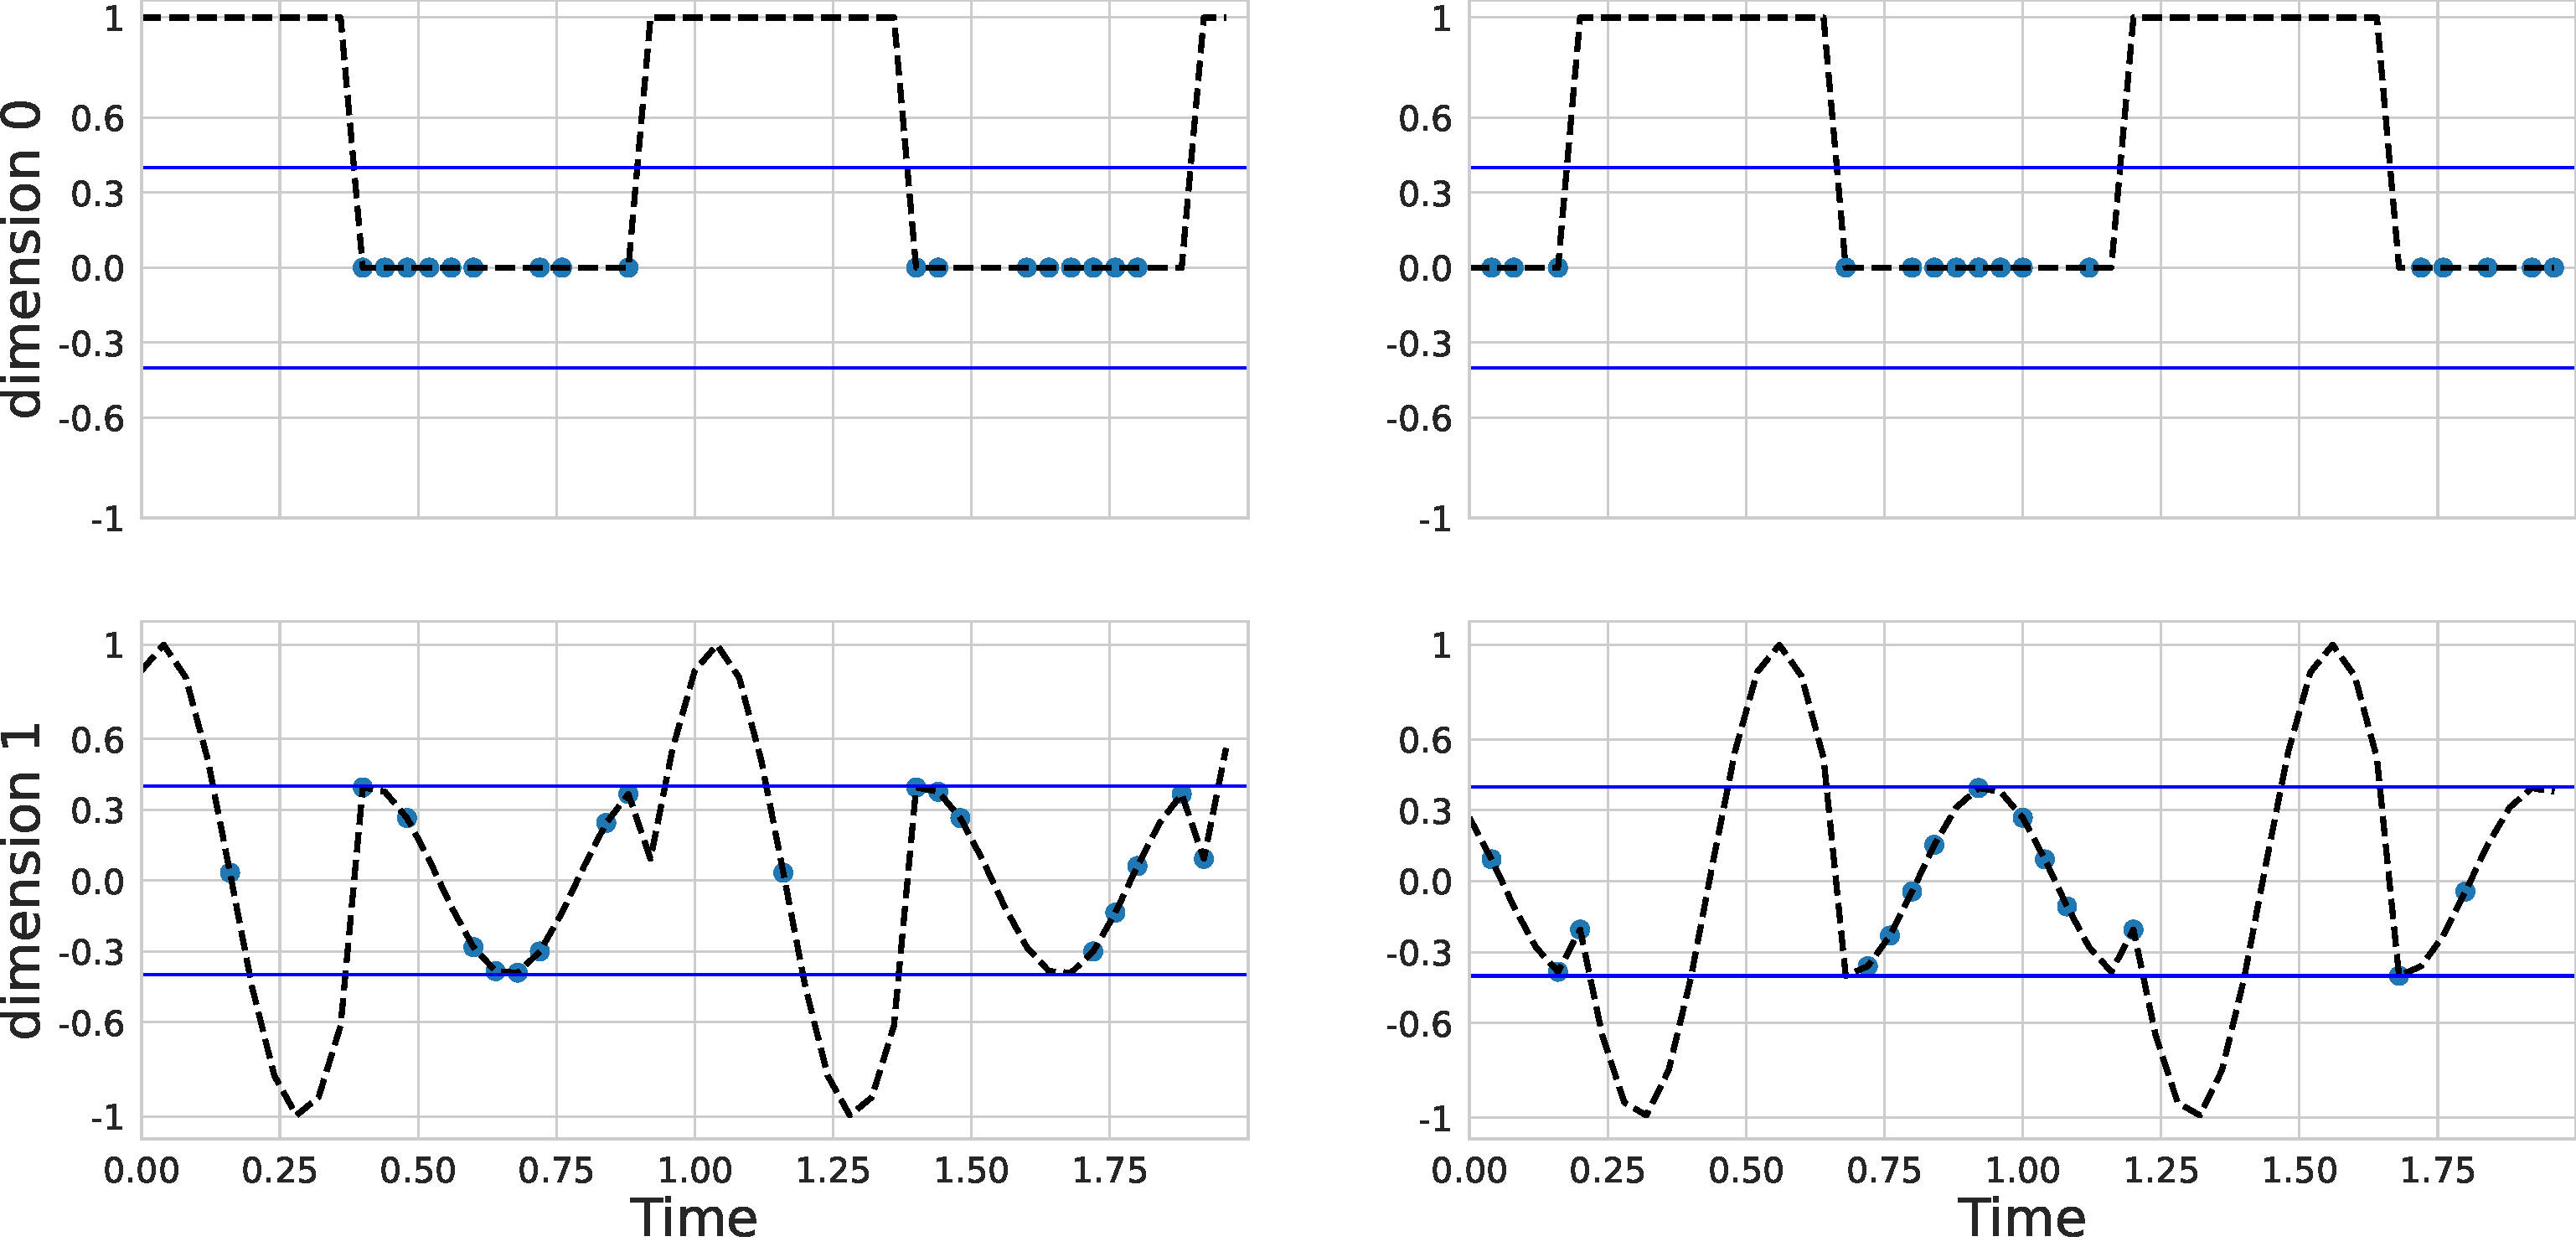
\includegraphics[width=0.9\textwidth]{content/chapters/irregular_time_series_data_driven_missingness/figures/toy_data.pdf}
    \caption[Examples of generated sequences for the synthetic task]{Two examples of generated sequences for the synthetic task. The dashed black lines represent the true data-generating process. The circular dots represent the observations at irregular timepoints. To incorporate data-dependent missingness, the probability of observing a value within the solid blue lines is 0.6; outside the lines is $p_{\text{S}}=0.0006$.}
    \label{fig:toy_example_sequences}
\end{figure}
